\subsection{Parameter Tuning}
The parameter tuning is important to the test because if not tuned correctly, the preprocessing methods will make the classification worse.
It was therefore decided to test the individual methods one by one and to possibly find the best setting.

\subsubsection{Raw Performance}
The parameter tuning for the pure K-NN is performed using the dataset of G3M2.
This was done because using a single persons dataset alone creates a clearer change in performance when comparing the scores.
Furthermore the reduced dataset makes it possible to test a larger set of parameters in less time.
The dataset was split in a $90\%/10\%$ split for training and test respectively.

To find the optimal value for $K$, figure \ref{fig:k_success}.

\begin{figure}[H]
\centering
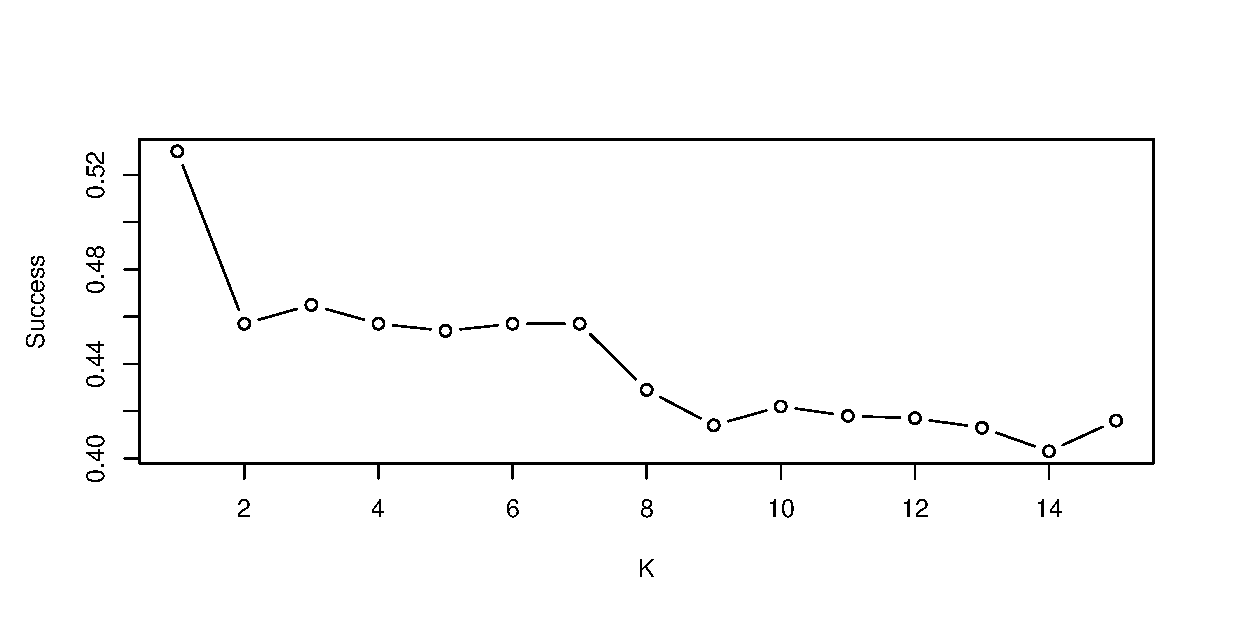
\includegraphics[width = 0.95 \textwidth]{graphics/knn_raw_success}
\caption{Success for K-NN with no preprocessing used.}
\label{fig:k_success}
\end{figure}

The best value for $K$ can from figure \ref{fig:k_success} be found to be $K = 1$.
For further test the value of $K = 1$ will hence be applied.
The same dataset is also for a range of the first initiating tests.


\subsubsection{Smoothing}
\label{sec:knn_smooth}
To find the best filter, the Gaussian filer is used.
As described earlier in section \ref{sec:smoothing}, then the Gaussian filter only has two parameters.
These are the kernel size and sigma.
When varying the sigma and kernel size, the contour in figure \ref{fig:cont_smooth_gaus_knn} is gained.

\begin{figure}[H]
\centering
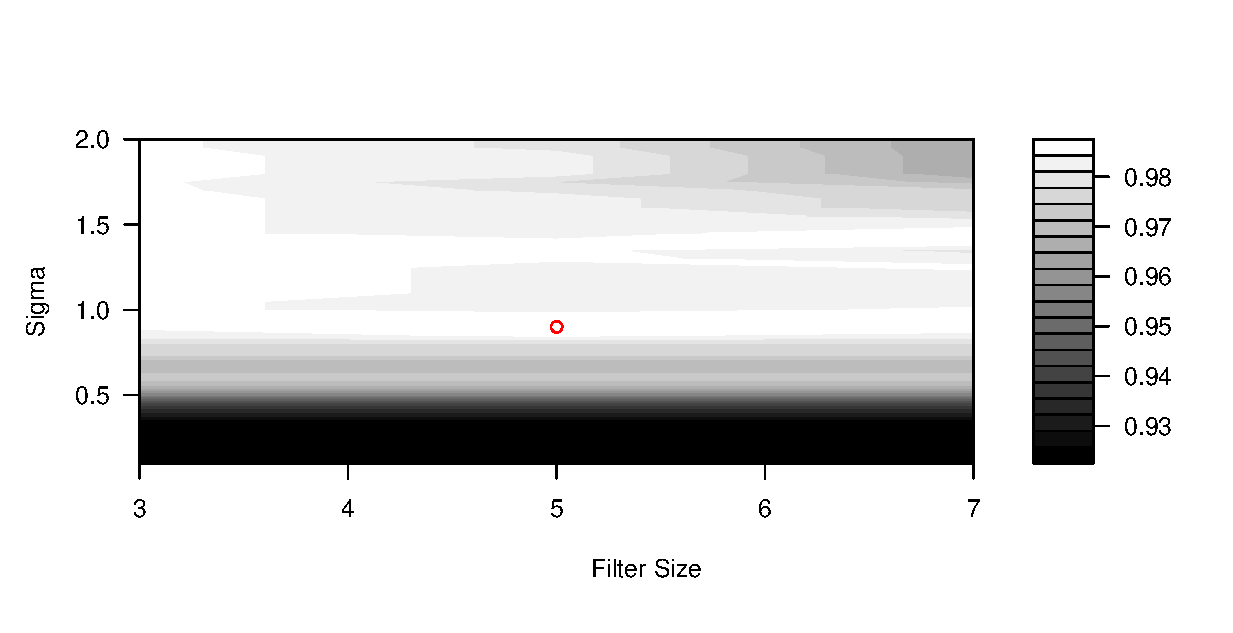
\includegraphics[width = 0.95 \textwidth]{graphics/knn_smooth_cont}
\caption[Success for K-NN with smoothing and PCA.]{Success for K-NN when the image is smoothed using a Gaussian filter with different kernel sizes and sigma values.}
\label{fig:cont_smooth_gaus_knn}
\end{figure}

The best point in figure \ref{fig:cont_smooth_gaus_knn} is highlighted with the red circle.
This is at $\sigma = 0.9$ and a kernel size of five.
This sigma and kernel size will hence be the one used onwards in this section when smoothing is done on the data before using K-NN.


\subsubsection{Principle Component Analysis}

The PCA was computed on the same dataset as in section \ref{sec:knn_smooth}.
The test where done on both the dataset with and without smoothing.
The result of plotting the number of PC versus the success and time taken to perform K-NN is seen on figure \ref{fig:plot_pca_knn}.

\begin{figure}[H]
\centering
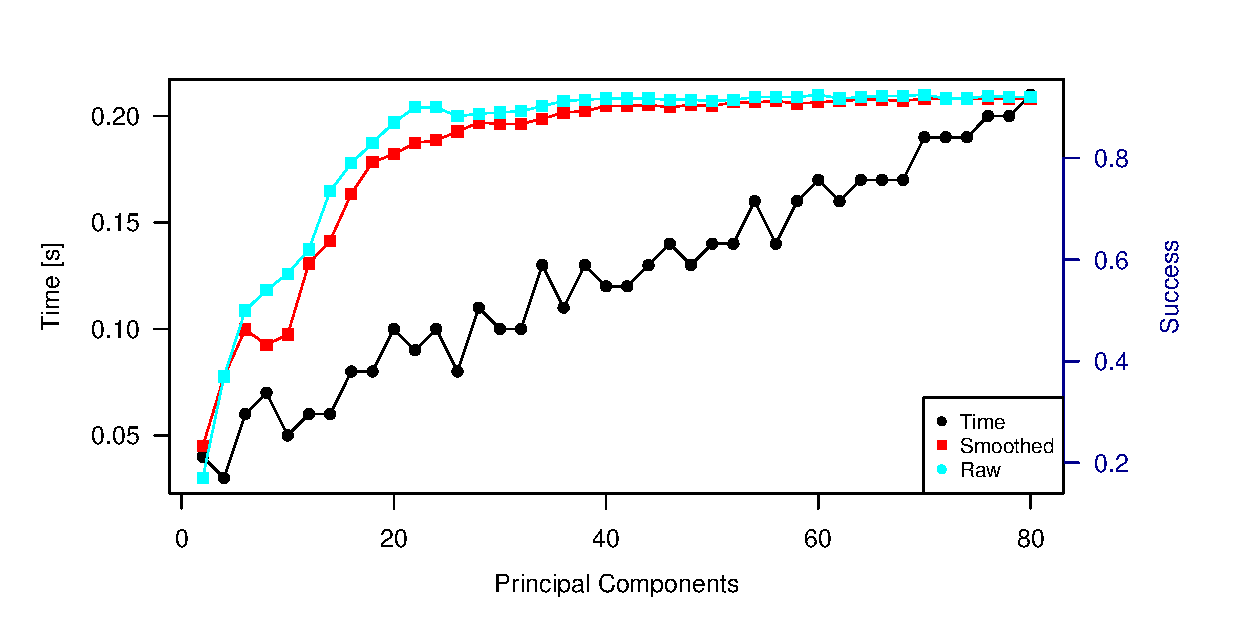
\includegraphics[width = 0.95 \textwidth]{graphics/knn_pc}
\caption{Success for K-NN for varying numbers of PC and sigma.}
\label{fig:plot_pca_knn}
\end{figure}


%Calculating with less data will result in a faster computation time.
%However, choosing too few PC results too few features left to compare.
%To see how the performance and the timing scales both are shown in figure \ref{fig:pca_timing_lukas} and \ref{fig:pca_timing_nikolaj}. K was chosen to be 10.
%In figure \ref{fig:pca_timing_lukas} the performance seems to be the same regardless of how many PC is chosen. As long as there are more than 60 the performance will be the same.
%On the test done on Group member 1 the performance is worse which means the digits are less uniform. 
%Here the success rate has a peak with a low set of attributes so there must be some confusion that gets sorted out. 
%Both test were run with 100 DPI. The percentage of successful predictions is also measured with the same data.
%The timing was measured on the same computer so the difference should not be very large. 

%To get a closer look at how the PCA performs the data from G3M2 was tested against the rest of the class. 
%The K was chosen to be 10. 
%The data is shown in figure \ref{fig:pca_success}.
%The performance is getting worse as more features are considered.


From figure \ref{fig:plot_pca_knn}, it was decided to use 40 PC.
This point was chosen because it efficiently reduces the dimensions of the dataset, but also has a descend success rate for the K-NN both with and without smoothing.
Furthermore the elbow-point is passed and no significant gain is gathered from taking more PC, compared to the timing advantage.



\subsubsection{Z-Score}
Z-score can be applied in a different number of ways.
This includes before PCA is made, after, both or not at all.
Furthermore this can be expanded to be used with and without smoothing and PCA.
This gives rise to 12 different ways in which the data can be processed.
Using the parameters for K-NN, PCA and smoothing, then the success rate of the different preprocessing methods can be computed.

The computations are done using three different datasets.
Once the dataset from the previous tests are used, the result of such is seen in figure \ref{fig:knn_zscore_1}.

A reduced dataset mixed with all peoples dataset can be used.
This is created taking 100 and 50 data points from each person into the test and train set respectively for each character.
Only one dataset was created (no cross-referencing).
The result of this is seen in figure \ref{fig:knn_zscore_2}.

The are also completed on the hard problem.
Here only 100 data points from one persons data was selected as the test set and 50 from each of the remaining people for the training set, for each character.
This gave the result in figure \ref{fig:knn_zscore_3}.


\begin{figure}[H]
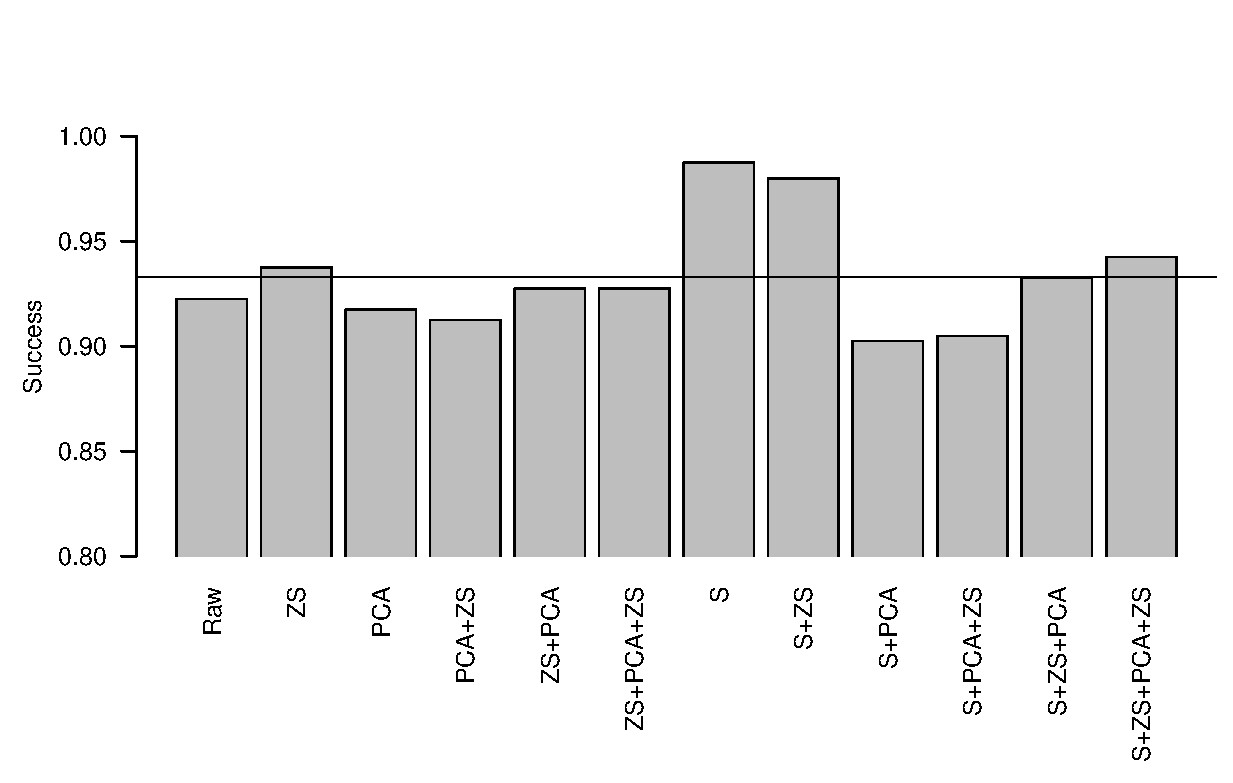
\includegraphics[width = 0.95 \textwidth]{graphics/knn_zscore_1}
\caption[Success for K-NN with different preprocessing schemes. Simplified problem.]{Success for the K-NN algorithm for one persons dataset. Different preprocessing schemes used.
Where $S$ is smoothing, $ZS$ is z-score.
The preprocessing schemes are named in the same order as applied.}
\label{fig:knn_zscore_1}
\end{figure}

\begin{figure}[H]
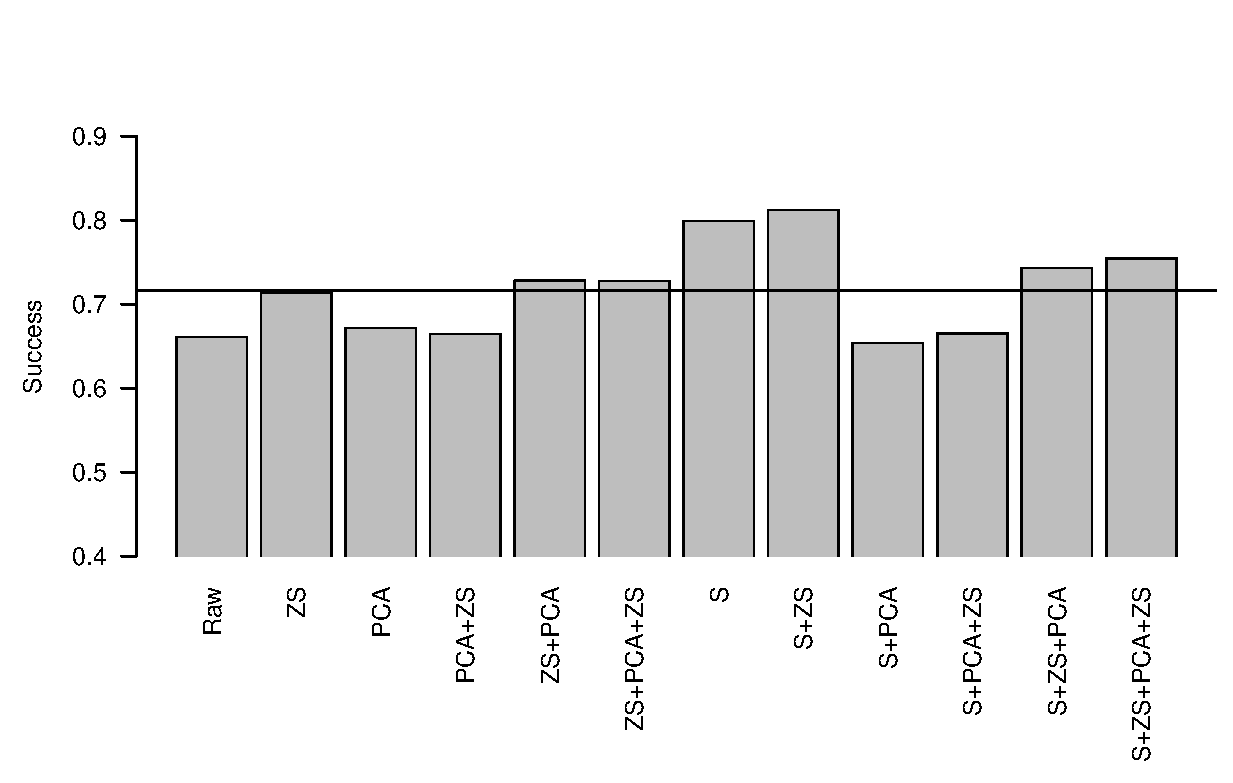
\includegraphics[width = 0.95 \textwidth]{graphics/knn_zscore_2}
\caption[Success for K-NN with different preprocessing schemes. Easy problem.]{Success for the K-NN algorithm for all peoples datasets mixed (easy problem no cross-referencing). Different preprocessing schemes used.
Where $S$ is smoothing, $ZS$ is z-score.
The preprocessing schemes are named in the same order as applied.}
\label{fig:knn_zscore_2}
\end{figure}

\begin{figure}[H]
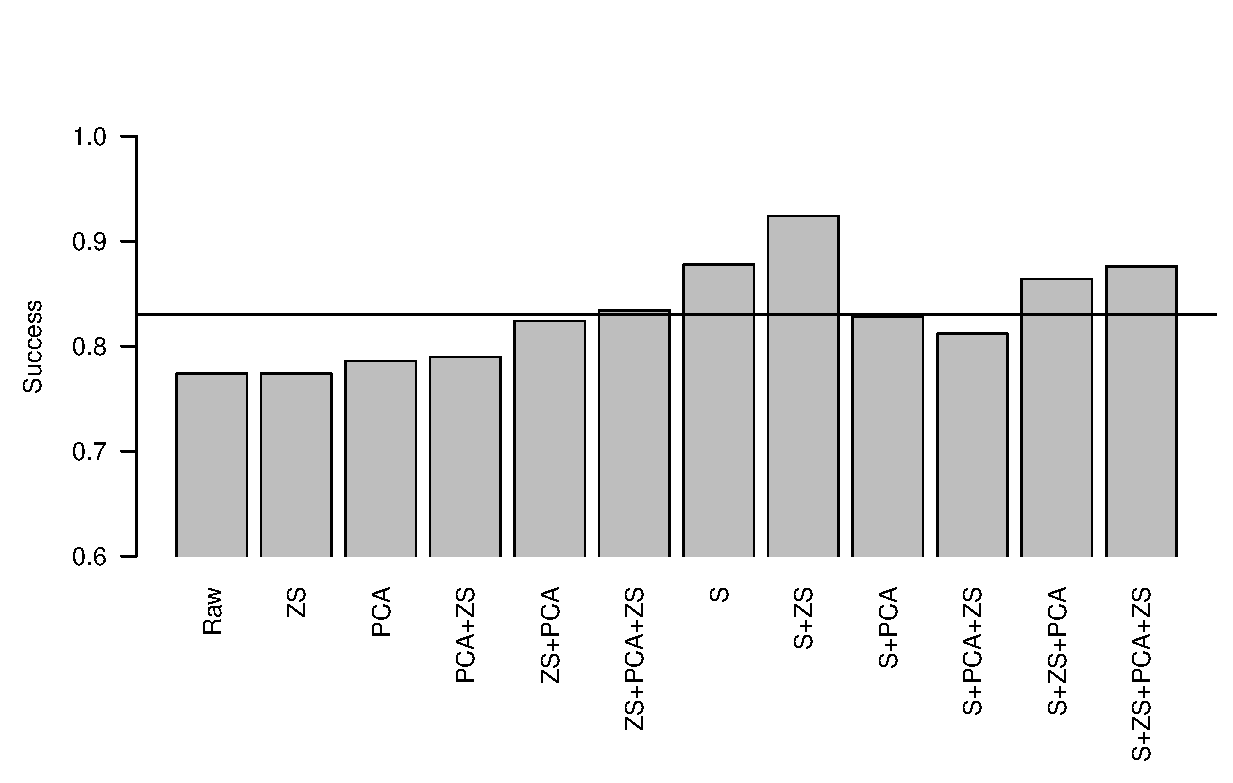
\includegraphics[width = 0.95 \textwidth]{graphics/knn_zscore_3}
\caption[Success for K-NN with different preprocessing schemes. Hard problem.]{Success for the K-NN algorithm for one person vs the rest (hard problem for G3M2 only). Different preprocessing schemes used.
Where $S$ is smoothing, $ZS$ is z-score.
The preprocessing schemes are named in the same order as applied.}
\label{fig:knn_zscore_3}
\end{figure}


As expected, all the test with PCA perform worse than those without as the dataset is heavily reduced.

To decide further which of the methods to use, then the timing of two best methods will be considered next.
%Because of the reduced computational time when using PCA, it is chosen to use one of the methods including PCA.
%Furthermore, then the success rate drop by using PCA is not of such a significant level that PCA is not beneficial.
%
%Considering the three figures \ref{fig:knn_zscore_1}, \ref{fig:knn_zscore_2} and \ref{fig:knn_zscore_3}, then it was chosen to use preprocessing scheme with smoothing and z-score both before and after PCA.
%This was chosen as it gives the highest success of all the schemes including PCA.


\subsection{Timing}

The two best methods where found to be the raw dataset with smoothing and z-score only and the dataset with smoothing, z-score and PCA applied.
To find the best of the two, the computation time is considered.
The time taken the compute the preprocessing and classification of the test data was hence measured.
Figure \ref{fig:knn_timing_comp} shows the result of the timing.

The dataset used is one in which the dataset of G3M2 is used as the test set and the remaining 19 peoples dataset is contained in the training set.


\begin{figure}[H]
\centering
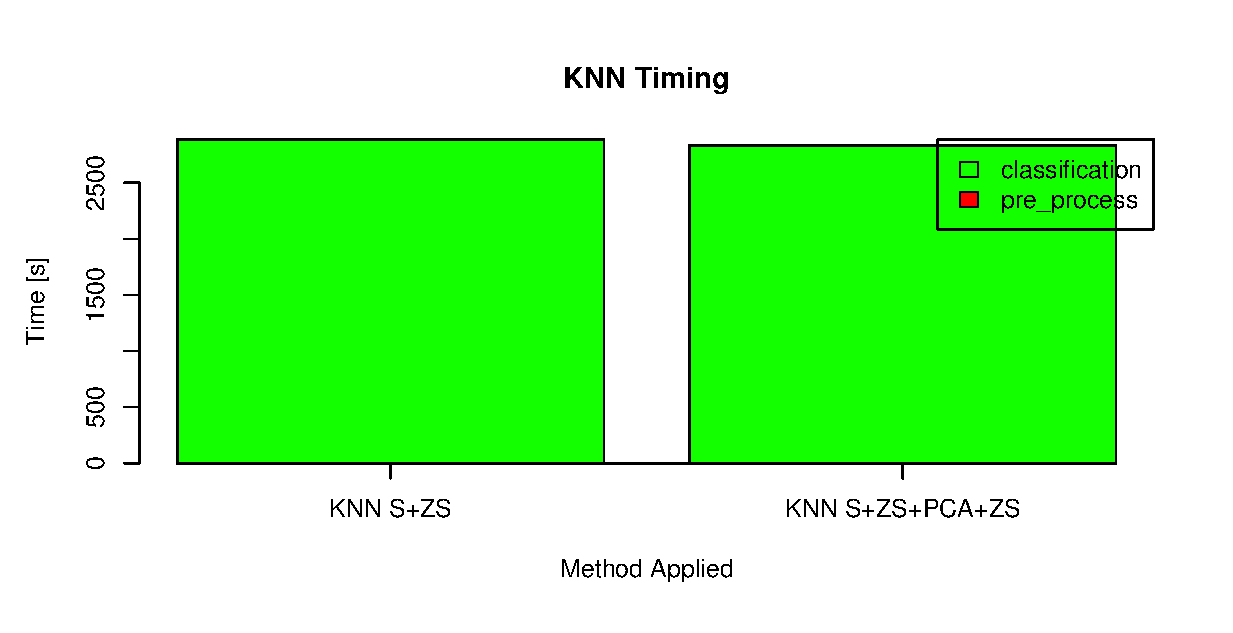
\includegraphics[width =  \textwidth]{graphics/compare_timing_knn_smoothVSpca}
\caption[Time distribution for K-NN.]{Time distribution of the preprocessing and classification time of the KNN algorithm in the two run modes.}
\label{fig:knn_timing_comp}
\end{figure}

The timing was computed for both the preprocessing of the testing set and the thereafter following classification using the data generated.
As seen on figure \ref{fig:knn_timing_comp} then the data preprocessed with PCA is 100 times faster than the data which was only smoothed and normalized.
It was therefore decided to use the reduced dataset to reduce the time taken to compute the classifications.


\subsubsection{Performance}

To test the overall performance with the final parameters, both confusion tables and success using K-NN with the beforehand decided preprocessing was computed.
Both the hard problem and the easy problem was computed.

The easy problem is the one in which the data from the different people is divided into a 90\%/10\% split, training and test respectively.
The test and training sets of each person are then combined.
This was done for ten cross-validation runs.
The result of such procedure can be seen in figure \ref{fig:knn_succ_final_easy}, where the success for the ten runs is shown in a boxplot, and figure \ref{fig:knn_conf_final_easy} shows the overall confusion matrix for all ten runs combined.


\begin{figure}[H]
\centering
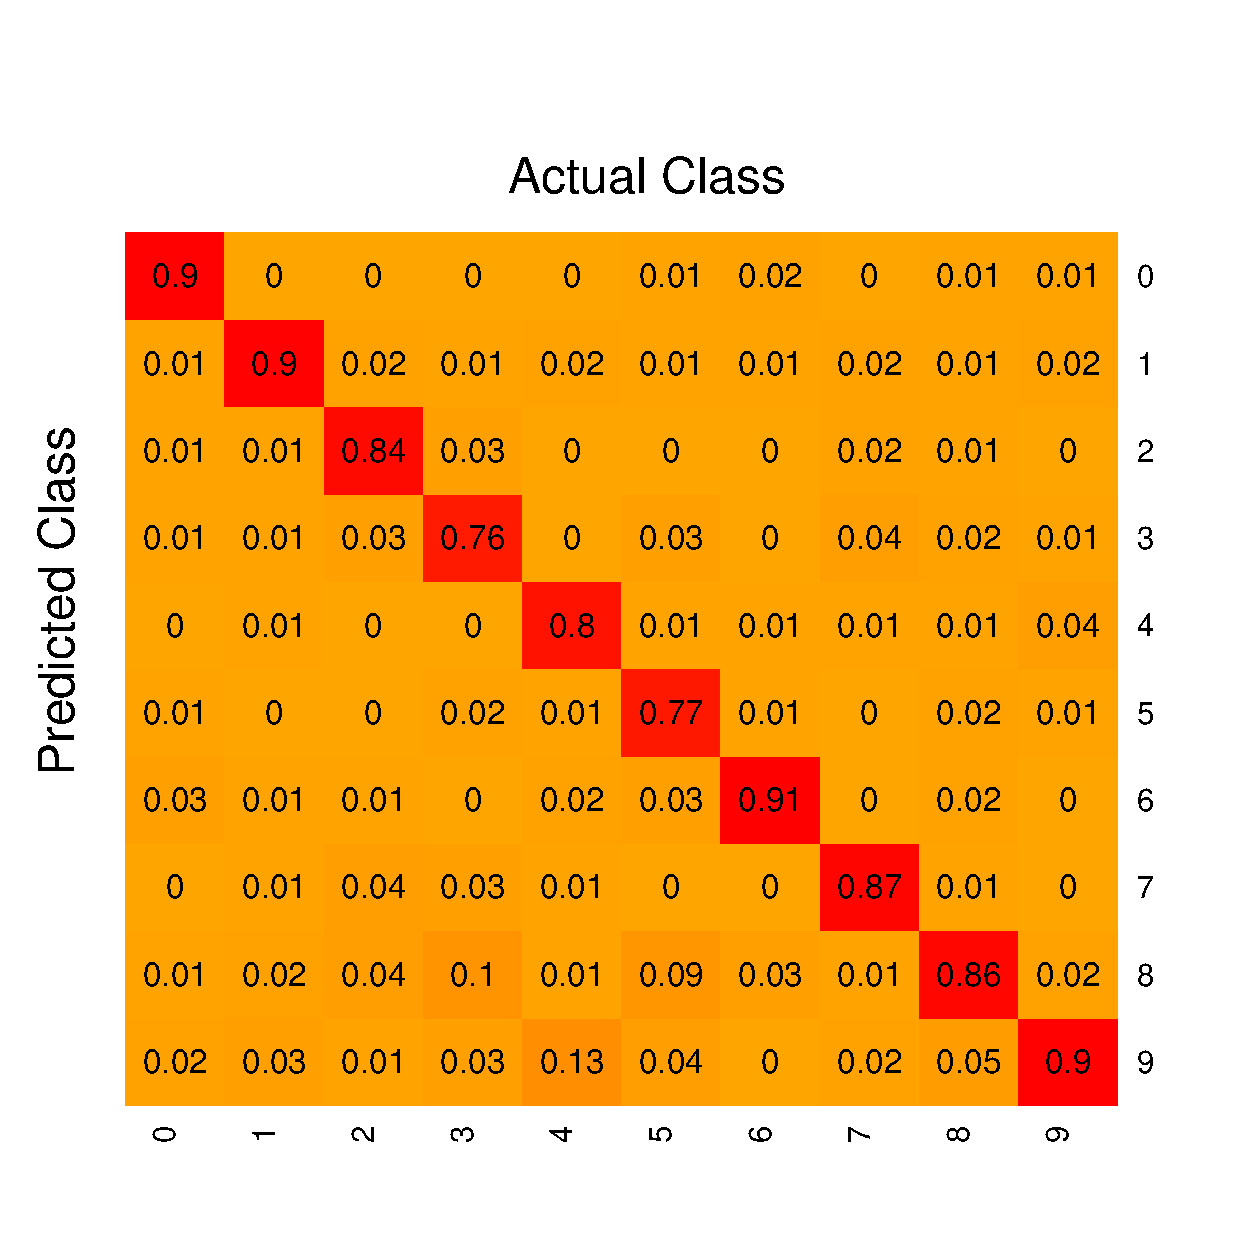
\includegraphics[width = 0.65 \textwidth]{graphics/knn_confusion_bestparam_easy}
\caption[Confusion table for the easy problem.]{Confusion table of the best parameter setting, for the easy problem with ten cross referencing runs.}
\label{fig:knn_conf_final_easy}
\end{figure}


\begin{figure}[H]
\centering
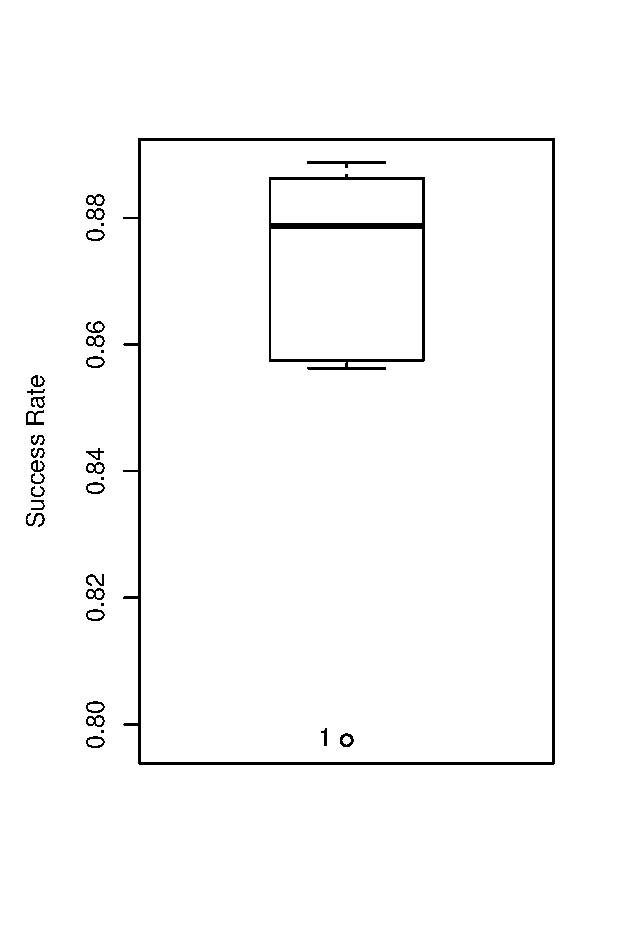
\includegraphics[width = 0.9 \textwidth]{graphics/knn_final_full_easy}
\caption[Success of K-NN on the easy problem.]{Success for the easy problem using ten cross referencing runs.}
\label{fig:knn_succ_final_easy}
\end{figure}


The hard problem is the one in which one persons test data was used as the test data alone and the remaining peoples put together in the training set.
This was done for all people with all the data present, such that each person once was used as the test set.
The success of such a process is seen in figure \ref{fig:knn_succ_final_hard} and figure \ref{fig:knn_conf_final_hard} shows the overall confusion table, when the confusion tables of each run was put together.


\begin{figure}[H]
\centering
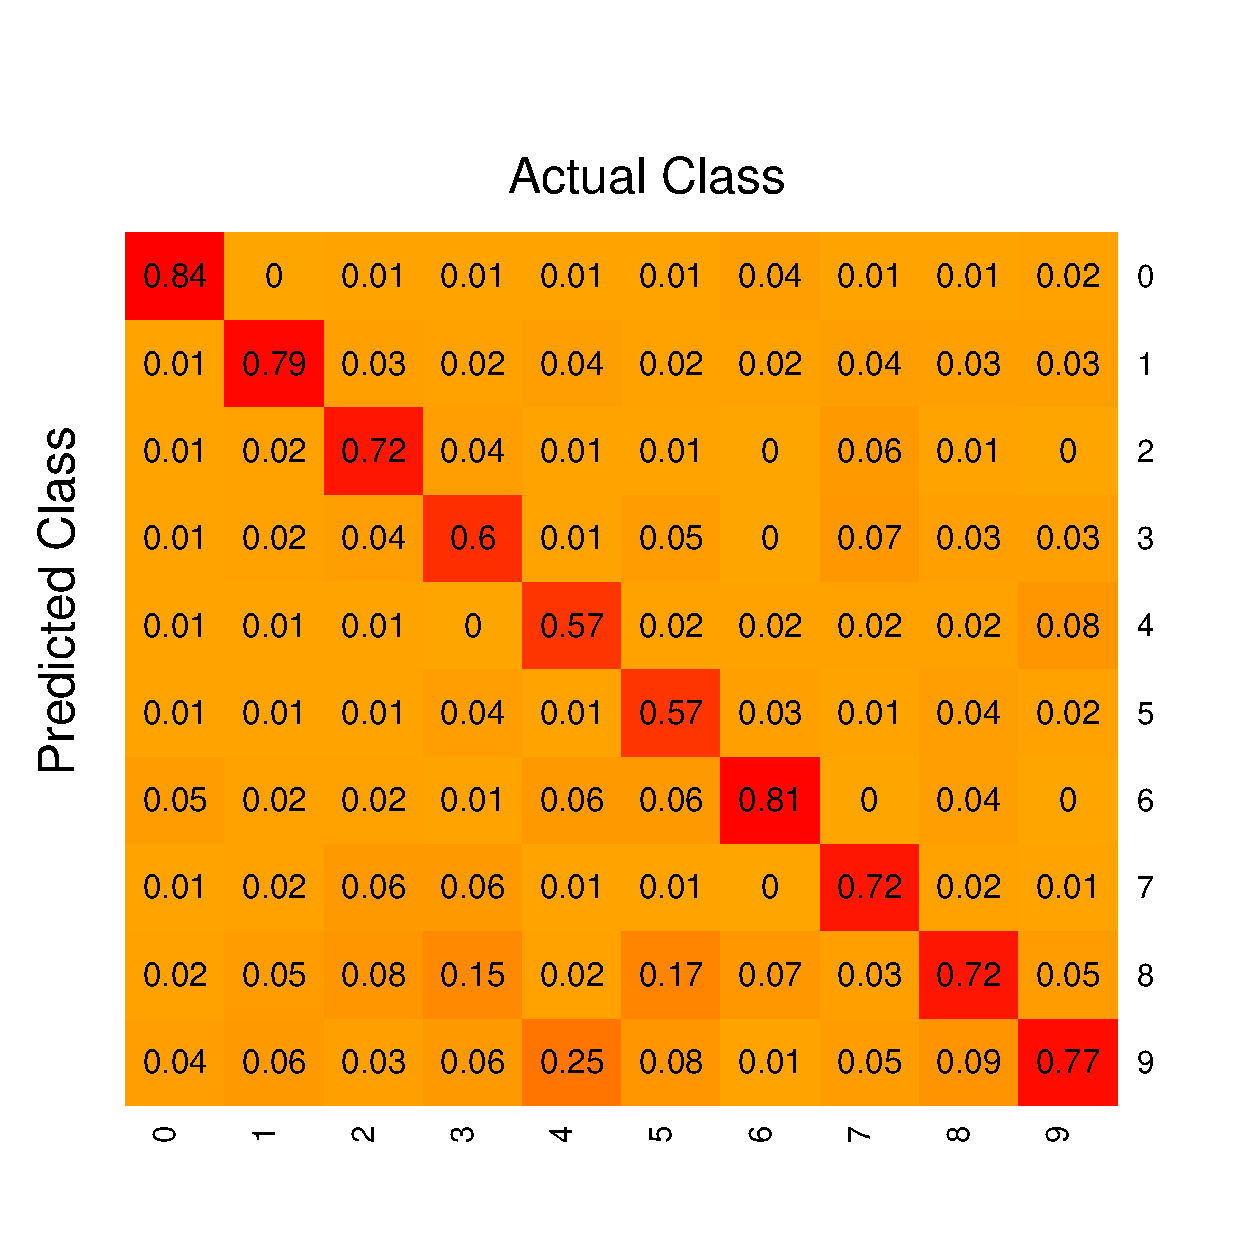
\includegraphics[width = 0.65 \textwidth]{graphics/knn_confusion_bestparam_hard}
\caption[Confusion table for the hard problem.]{Confusion table with all the best parameters for the full dataset difficult problem with the confusion tables for the different runs combined.}
\label{fig:knn_conf_final_hard}
\end{figure}



With a mean of $70.99\%$ and variance of  $117.81\%^2$, then the hard problem clearly performs worse than the easy problem with $85.07\%$ mean and $3.59\%^2$ variance.
The general tendency is that the greatest error comes from the '3' and '5' often being detected as '8', and the '4' being classified as a '9'.
These two errors account for 5.7\% and 3.3\% of the error in hard and easy problem respectively, and is hence more than 1/6 in the two classification problems.
This is, however, expected as the characters of confusion have great similarity compared to any other class in the dataset.

\begin{figure}[H]
\centering
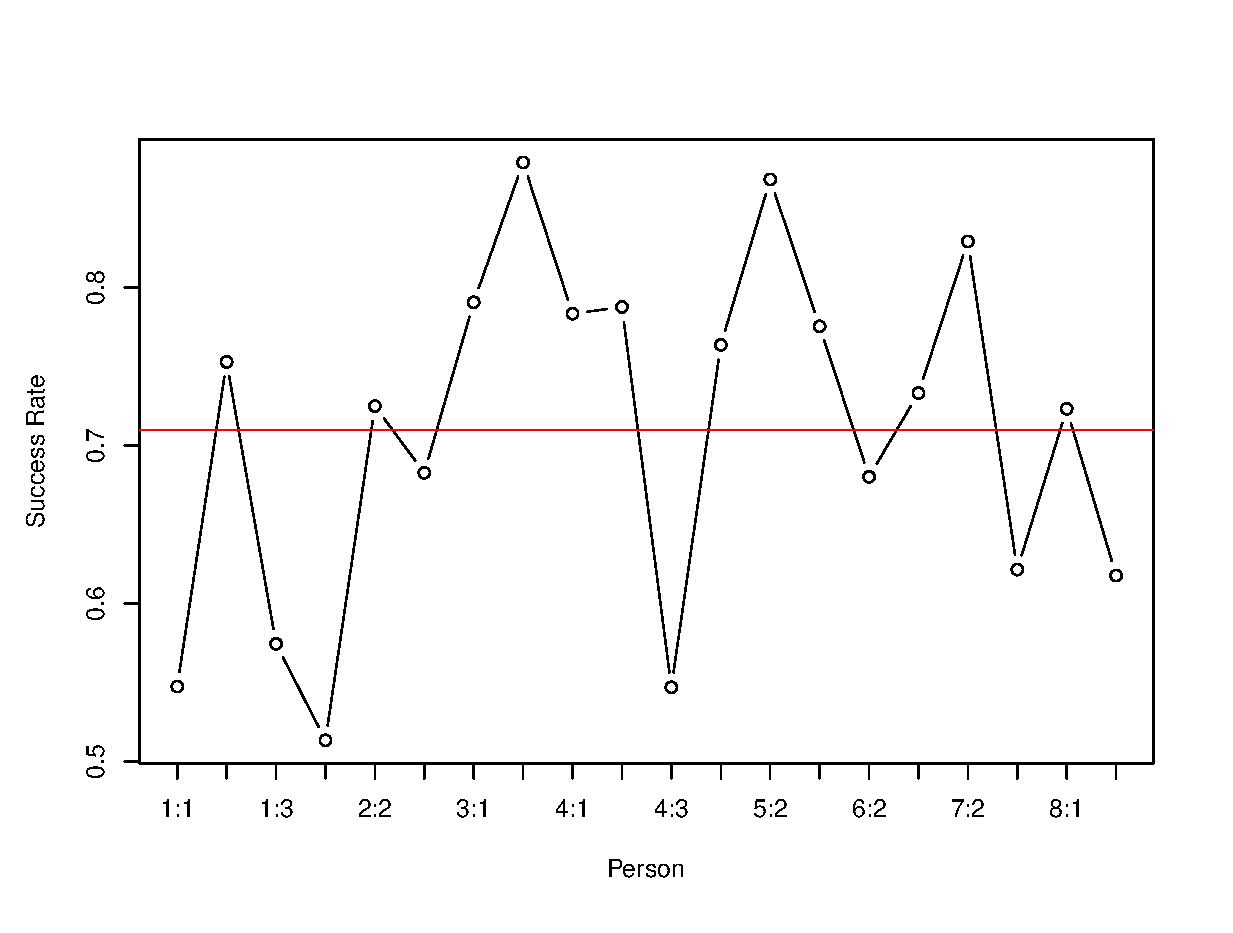
\includegraphics[width = 0.95 \textwidth]{graphics/knn_final_full_hard}
\caption[Success for K-NN for the hard problem.]{Success for the hard problem for each person.
The y-axis values represents the "Group:Member" number used as the test set.}
\label{fig:knn_succ_final_hard}
\end{figure}